% Source of Fig. 1 (the pipeline diagram). Regenerate the PNG with build.sh, which compiles
% this file and renders it. Labels: "reasoning subnetwork" replaces "reasoning tower"
% (Frank's comment C19, 23 October 2026); SAM 2 spelled as in the references.
\documentclass{article}
\usepackage[paperwidth=22cm,paperheight=10cm,margin=0.3cm]{geometry}
\usepackage{tikz}
\usetikzlibrary{arrows.meta,positioning,calc}
\pagestyle{empty}
\begin{document}
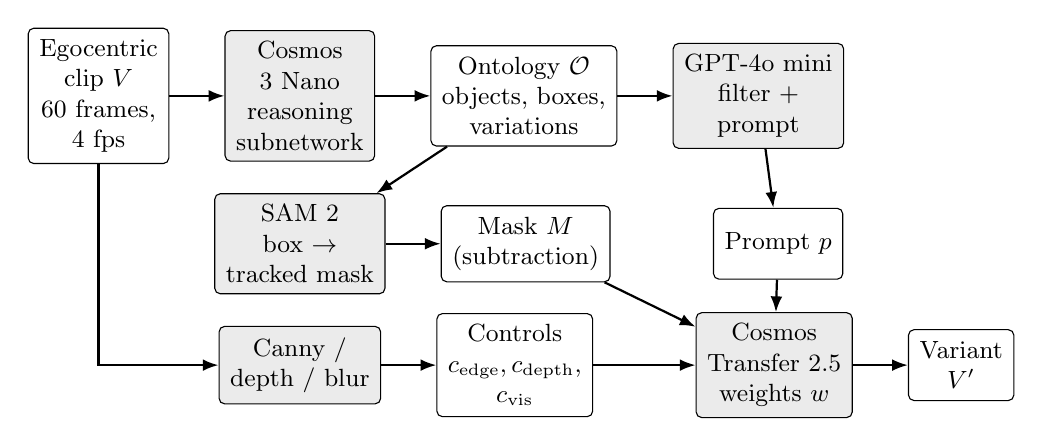
\begin{tikzpicture}[
  node distance=4mm and 7mm,
  box/.style={draw, rounded corners=2pt, align=center, font=\small, inner sep=4pt, minimum height=9mm},
  model/.style={box, fill=black!8},
  data/.style={box, fill=white},
  arr/.style={-{Latex[length=2mm]}, thick}
]
\node[data] (clip) {Egocentric\\clip $V$\\60 frames,\\4 fps};
\node[model, right=of clip] (reason) {Cosmos\\3 Nano\\reasoning\\subnetwork};
\node[data, right=of reason] (onto) {Ontology $\mathcal{O}$\\objects, boxes,\\variations};
\node[model, right=of onto] (llm) {GPT-4o mini\\filter +\\prompt};
\node[model, below=of reason] (sam) {SAM 2\\box $\to$\\tracked mask};
\node[data, right=of sam] (mask) {Mask $M$\\(subtraction)};
\node[data, right=of mask, xshift=6mm] (prompt) {Prompt $p$};
\node[model, below=of sam] (pre) {Canny /\\depth / blur};
\node[data, right=of pre] (ctrl) {Controls\\$c_{\mathrm{edge}}, c_{\mathrm{depth}},$\\$c_{\mathrm{vis}}$};
\node[model, right=of ctrl, xshift=6mm] (transfer) {Cosmos\\Transfer 2.5\\weights $w$};
\node[data, right=of transfer] (out) {Variant\\$V'$};
\draw[arr] (clip) -- (reason);
\draw[arr] (reason) -- (onto);
\draw[arr] (onto) -- (llm);
\draw[arr] (llm) -- (prompt);
\draw[arr] (onto) -- (sam);
\draw[arr] (sam) -- (mask);
\draw[arr] (clip) |- (pre);
\draw[arr] (pre) -- (ctrl);
\draw[arr] (ctrl) -- (transfer);
\draw[arr] (mask) -- (transfer);
\draw[arr] (prompt) -- (transfer);
\draw[arr] (transfer) -- (out);
\end{tikzpicture}
\end{document}
